\documentclass[19pt,a4paper]{article}
\usepackage{xeCJK}
\usepackage{amsmath}
\setmainfont{STSong}
\usepackage{geometry}
\geometry{left=2.5cm,right=2.5cm,top=2.5cm,bottom=2.5cm}
\setlength{\parindent}{4em}
\usepackage{graphicx}
\usepackage{float}
\title{思考题9}
\author{孟妍廷2015202009}
\date{2017年12月2日}

\begin{document}
\maketitle
a.证明:首先明确定义:在深度优先森林中,v是u的子结点当且仅当v在u为灰色的时间段里被发现\\
以下图为例:
\begin{figure}[H]
\centering
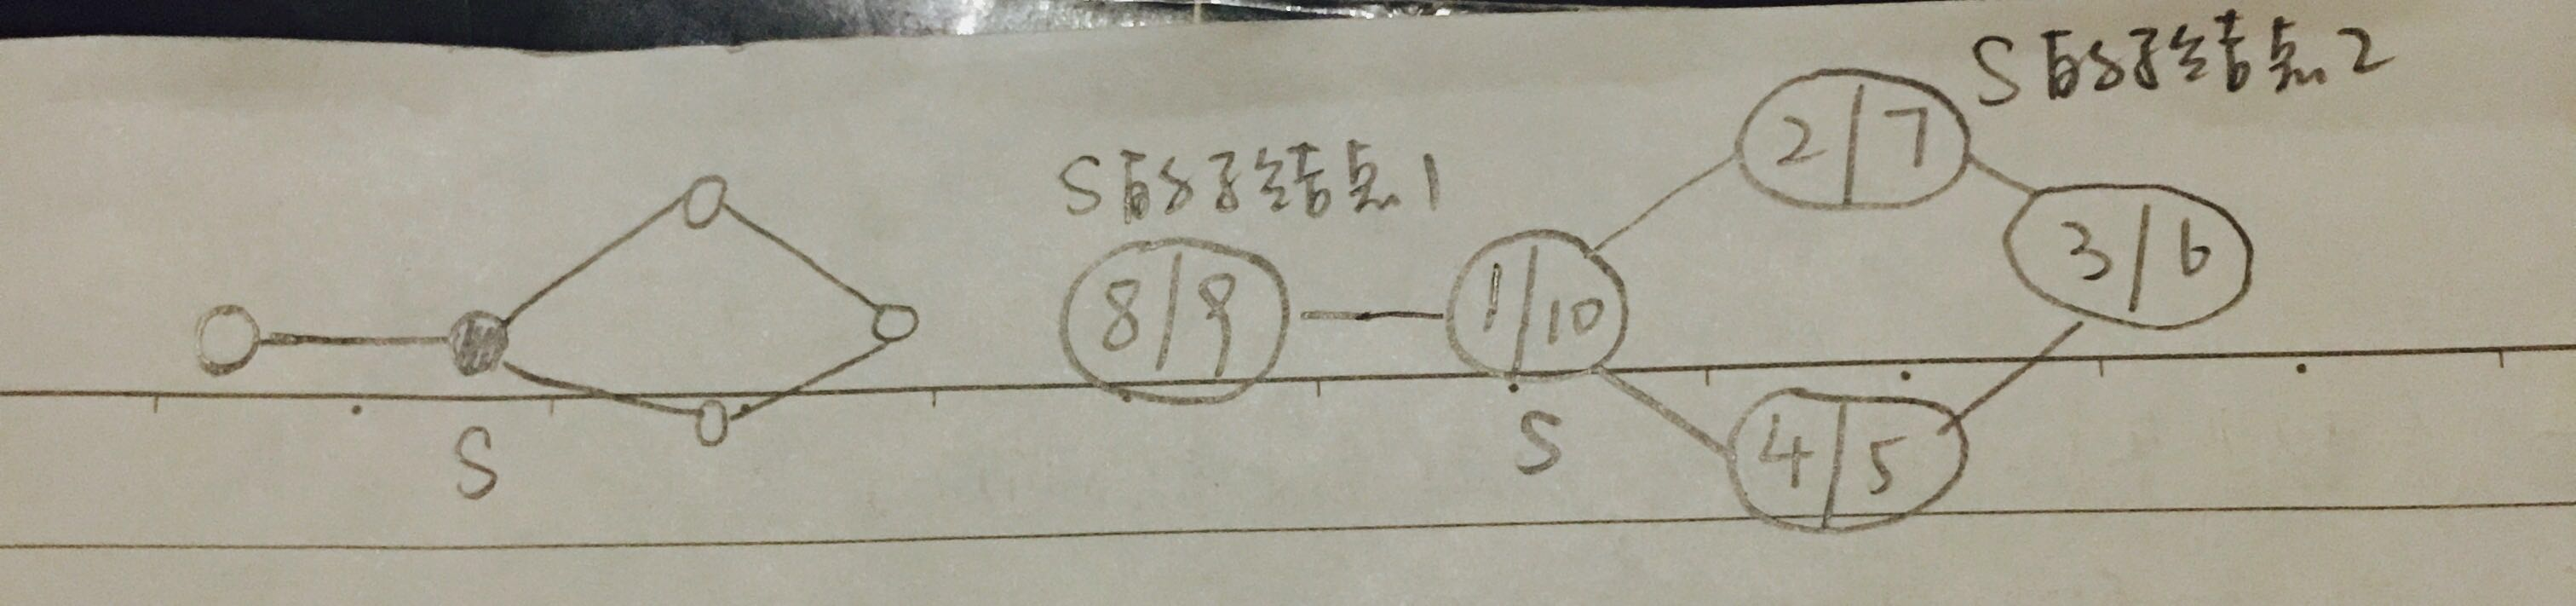
\includegraphics[scale=0.1]{1.jpeg}
\end{figure}
\indent s为衔接点,且s为$G_\pi$的根结点,s有两个子结点说明s能够发现两个处于不同环路的结点或能发现一个单独结点和一个处于环路的结点,所以s一定为衔接点,衔接点作为根结点一定有两个子结点
\\
\indent b.证明:以下图为例:
\begin{figure}[H]
\centering
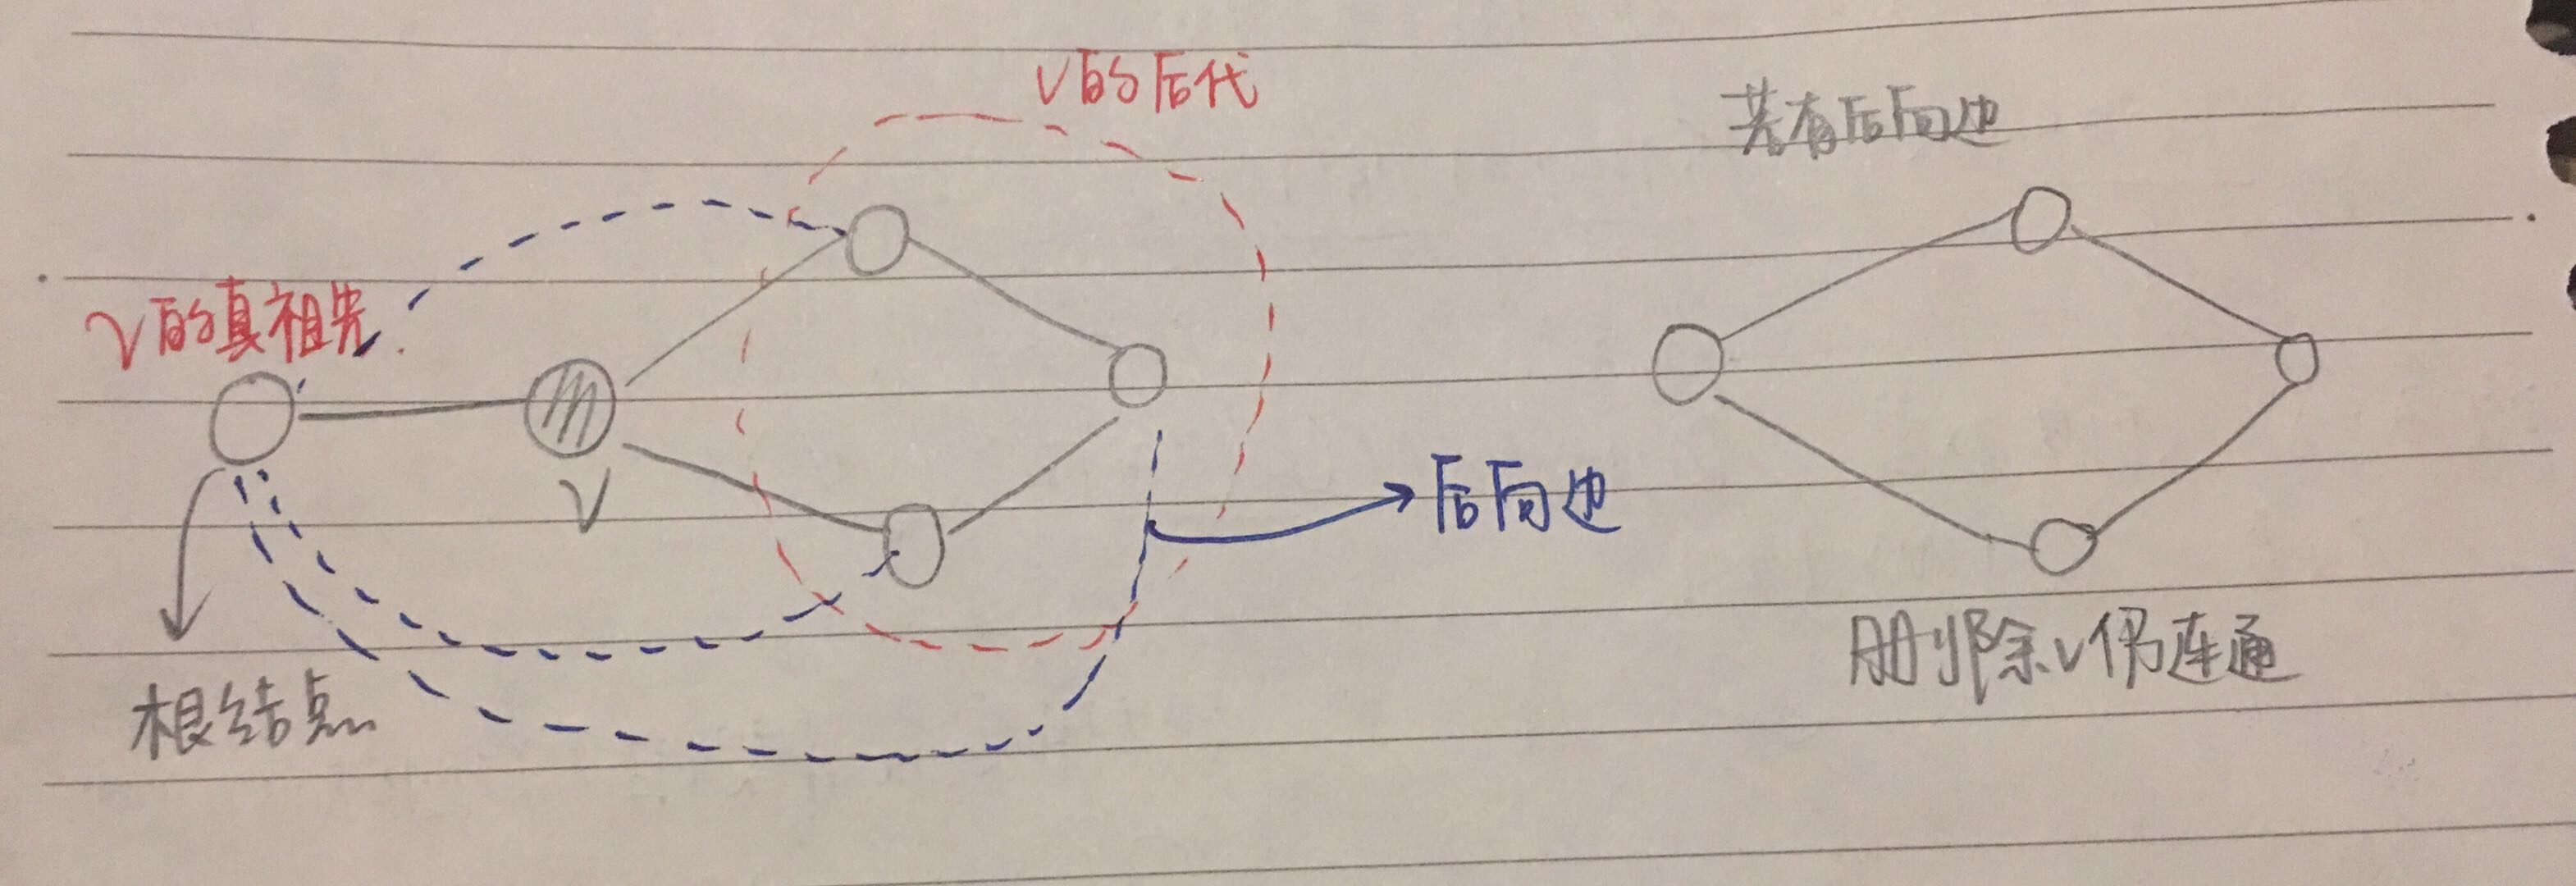
\includegraphics[scale=0.1]{2.jpeg}
\end{figure}
\indent 节点v为衔接点,且v不是$G_\pi$的根结点,则v的祖先与v的后代应该处于不同的环路,若有v的后代指向v的祖先的后向边,v就不可能是衔接点了。
\\
\indent c.首先明确定义:v.d是结点v第一次被发现的时间,即为第一时间戳。由b的证明可知,不存在连接两个环路的后向边,所有的后向边至多只能指向这一环路中的衔接点,但又由于环路中一定存在后向边,所以每一个环路中的结点的v.low应该都等于深度优先搜索过程中该环路中被发现的第一个点的v.d\\
修改DFS-VISIT算法来计算所有结点的v.low值:\\
\indent $DFS-VISIT(G,u)\\
\indent\quad time=time+1\\
\indent\quad u.d=time\\ 
\indent\quad u.color=GRAY\\
\indent\quad for\ each\ v\in G:Adj[u]\\
\indent\quad\quad if\ v.color ==WHITE\\
\indent\quad\quad\quad v.\pi=u\\
\indent\quad\quad\quad DFS-VISIT(G,v)\\
\indent\quad\quad if\ v.color==GRAY//后向边\\
\indent\quad\quad\quad while\ u\ne v\\
\indent\quad\quad\quad\quad u.low=v.d\\
\indent\quad\quad\quad\quad u=u.\pi\\
\indent\quad u.color=BLACK\\
\indent\quad time=time+1\\
\indent\quad u.f=time$\\
\\
\indent d.与c的逻辑类似,由于每一个环路中的结点的v.low应该都等于深度优先搜索过程中该环路中被发现的第一个点的v.d,而衔接点间的连线应该是两个环路的唯一通路,所以应该在c计算出每一个几点的v.low之后,遍历所有的边,检查每条边的端点的v.low,若对于某条边(u,v),若$u.d\ne v.d$且u,v均还有其他的边,说明u,v处于两个不同环路中而不是单独结点,则u,v均为衔接点。\\
\indent 因此遍历即可在O(E)时间内得到所有衔接点\\
\\
\indent e.证明:利用反证法,假设一条边是桥,且该条边位于一个简单环路中:\\
以下图为例:
\begin{figure}[H]
\centering
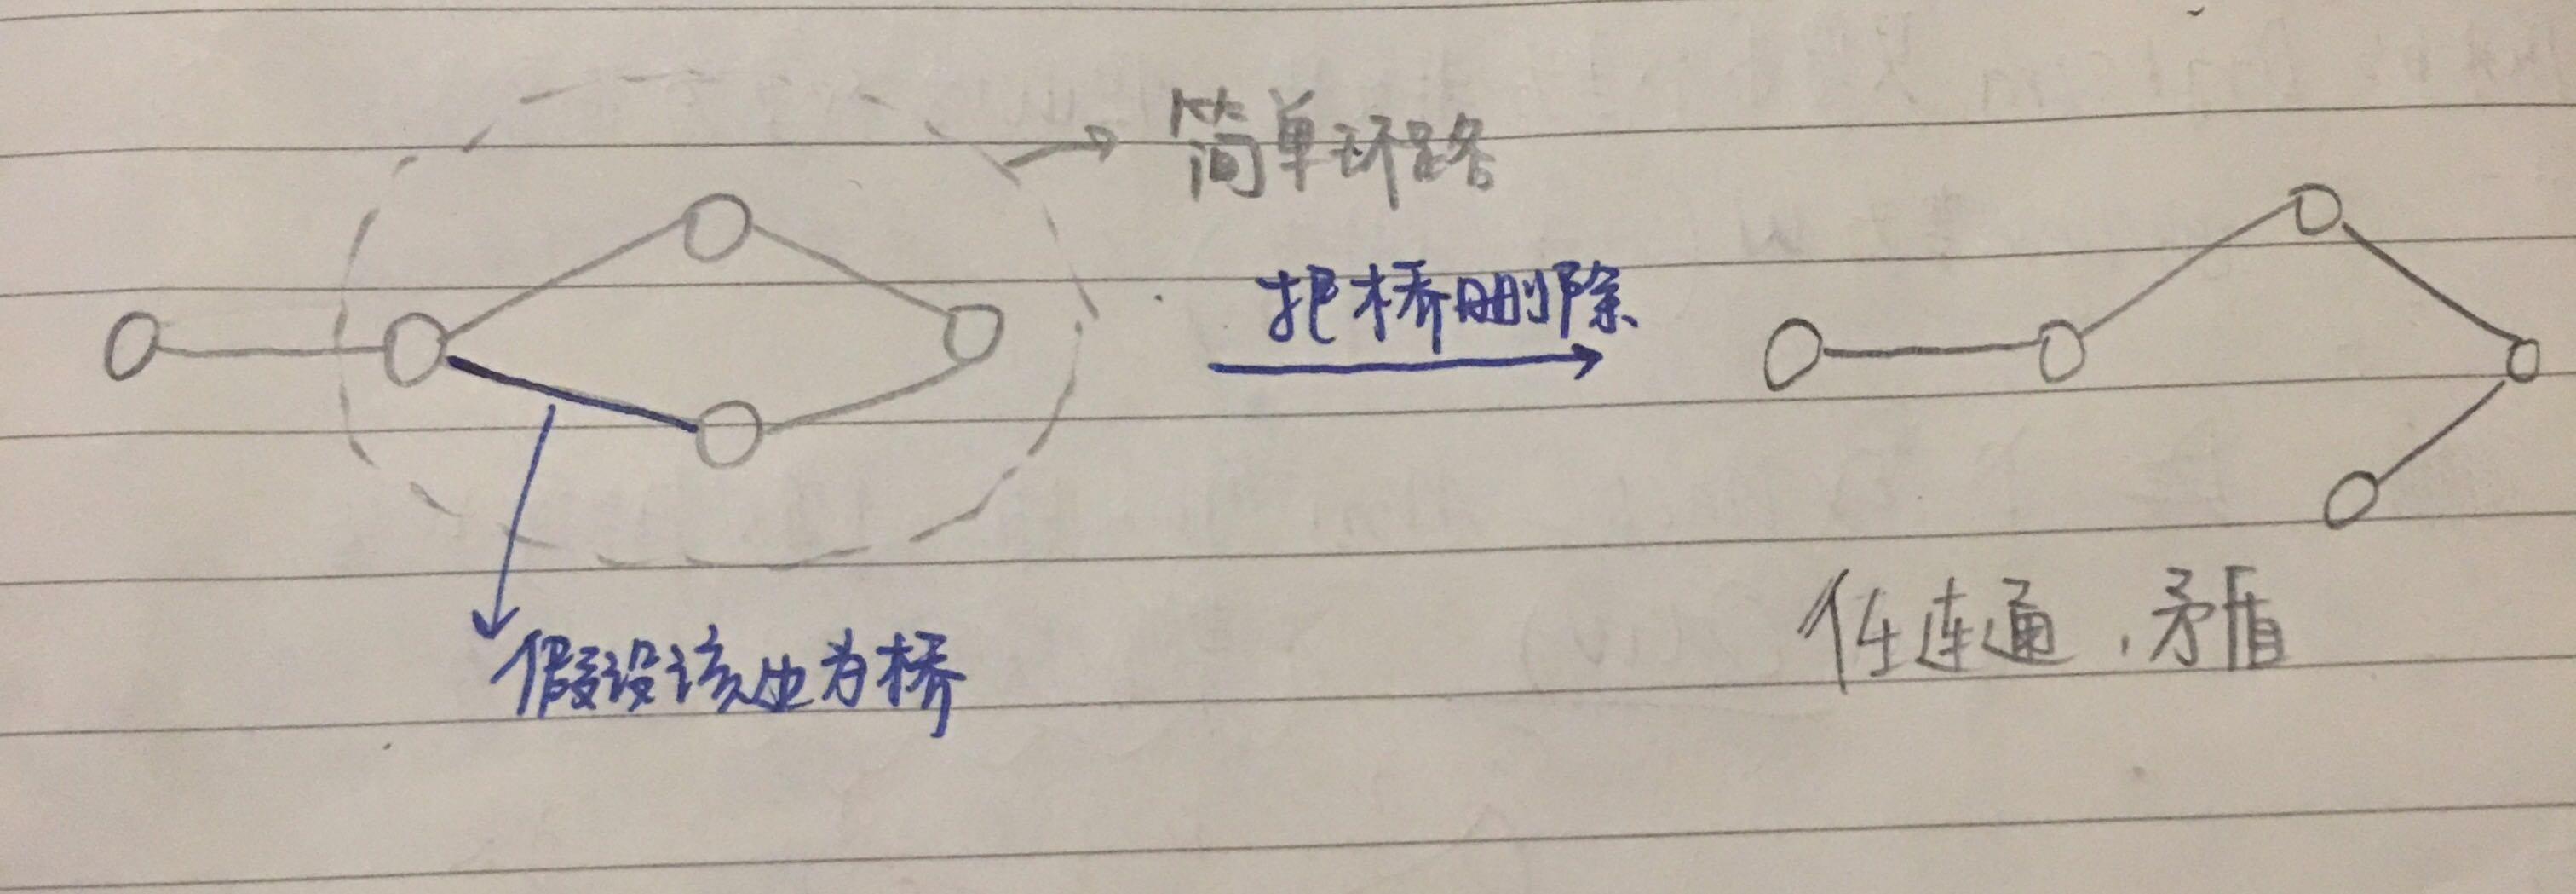
\includegraphics[scale=0.1]{3.jpeg}
\end{figure}
\indent 若某条边既为桥又处于环路,则把该桥删除之后图任然连通,不符合桥的定义,产生矛盾,故假设不成立。因此一条边是桥当且仅当改变不属于任何简单环路\\
\\
\indent f.由以上证明可知桥并不属于环路,而环路中所有点边的两个端点的v.low一定是相等的,所以算出桥的方法与找出衔接点的方法类似。故遍历所有的边,检查每条边的端点的v.low,若对于某条边(u,v),若$u.d\ne v.d$且u,v均还有其他的边,说明边(u,v)不处于环路中而是起到连接两个环路的作用,故(u,v)边为桥。
\indent 因此遍历即可在O(E)时间内得到所有桥。\\
\\
\indent g.证明:一个划分具有的性质是:在一个划分内,删除一条边不影响其连通性。\\
而已知删除桥后图就无法连通,而一个简单环路中删除一条边不影响连通性,而双联通分量中任意两条边都处于同一简单环路中,故G的双连通分量是G的非桥边的一个划分。\\
\\
\indent h.由以上分析可知,只有处于同一双连通分量的边的两端结点的v.low才相等,所以只用构造关于v.low的哈希函数来计算e.bcc即可。此时只用两条边处于同一双连通分量时它们的e.bcc才可能相等。

\end{document}

